\section{Ergebnisse}
\subsection{Fahrrad Datenblatt}

  Die folgenden Abschnitte beschreiben eine in Webots aufgebaute Simulation als digitalen Zwilling des realen Testfahrrads. Ziel ist, Masse-, Trägheits- und 
  Reibungsparameter sowie Sensor-/Aktorschnittstellen so realitätsnah zu spiegeln, dass das Fahrverhalten und die Reglerkopplung mit dem Prototyp übereinstimmen. 
  Auf Basis der ODE-Physik in Webots und der Controller-API (C/Python) wird die in der Hardware verwendete Architektur nachgebildet: eine schnelle innere 
  Balance-Schleife und eine langsamere, vision-gestützte MPC-Spurführung. Eine Supervisor-Instanz ermöglicht reproduzierbare Versuchsreihen, Resets und Logging, 
  sodass Parameterstudien und Kalibrierungen unter identischen Bedingungen erfolgen. Damit dient die Simulation als sichere Vorstufe für reale Fahrversuche und 
  als Referenz für die im Anschluss dokumentierten physikalischen Eigenschaften und Regelungsparameter.

  \begin{figure}[H]
    \centering
    
\includegraphics[width=1.0\textwidth]{figures/Datenblatt.png}  
    \caption{Datenblatt}
    \label{fig:datenblatt}
  \end{figure}
  
  \begin{itemize}
    \item \textbf{Masse und Schwerpunkt:} Der Rahmen des simulierten Fahrrads wiegt 3{,}5\,kg; zusammen mit den Rädern beträgt die Gesamtmasse ca. 5{,}1\,kg. 
    Der Schwerpunkt liegt etwa 5\,cm über dem Boden\gh, was ein stabiles Balanceverhalten begünstigt.
    
    \item \textbf{Trägheitssensor:} Im Webots--Modell ist der Trägheitssensor als Array in der Form
    \[
      [\,I_{xx}\; I_{xy}\; I_{xz}\; I_{xy}\; I_{yy}\; I_{yz}\; I_{xz}\; I_{yz}\; I_{zz}\,]
    \]
    angegeben. Für den Fahrradrahmen ergibt sich ein annähernd diagonal dominanter Trägheitstensor mit
    \(I_{xx}\approx I_{yy}=0{,}1\) und \(I_{zz}=0{,}05\,\mathrm{kg\,m^{2}}\)\gh. Der kleinere Wert um die Hochachse (Yaw-Trägheit) erleichtert schnelle 
    Lenkbewegungen; die Off-Diagonaleinträge sind Null, was bedeutet, dass die Hauptträgheitsachsen mit den Achsen des Modells ausgerichtet sind.
    
    \item \textbf{Räder:} Die beiden Räder haben einen Radius von 5{,}5\,cm und jeweils etwa 0{,}8\,kg Masse\gh. Durch die rotierende Masse entsteht ein 
    kleiner gyroskopischer Stabilisierungs-Effekt (Trägheitsmoment pro Rad ca. \(1\times10^{-3}\,\mathrm{kg\,m^{2}}\)), der zur Gesamtstabilität beiträgt, 
    aber aufgrund des geringen Werts nur begrenzten Einfluss hat\gh.
    
    \item \textbf{Reibungsparameter:} Die Radnaben besitzen eine viskose Lagerdämpfung (\texttt{dampingConstant} = 0{,}1) sowie Haftreibung (\texttt{staticFriction} = 0{,}1)\gh. 
    Diese Parameter simulieren Lagerveluste und verhindern z.\,B. ein freies Schwingen oder Durchrutschen der Räder im Stillstand. Zwischen Reifen und 
    Untergrund sorgt ein Coulomb-Reibungskoeffizient von etwa 0{,}8 für gute Traktion\gh; ein geringer Rückprallkoeffizient von 0{,}1 begrenzt die 
    Sprungelastizität des Reifenkontakts.
  \end{itemize}

  





\subsection{Teststrecken}
%------------------------------------------------------------------------------------------------
%------------------------------------------------------------------------------------------------
\subsubsection{Kurvenfahrt}
  \begin{wrapfigure}{r}{0.40\textwidth}
    \vspace{-0.8\baselineskip}
    \centering
    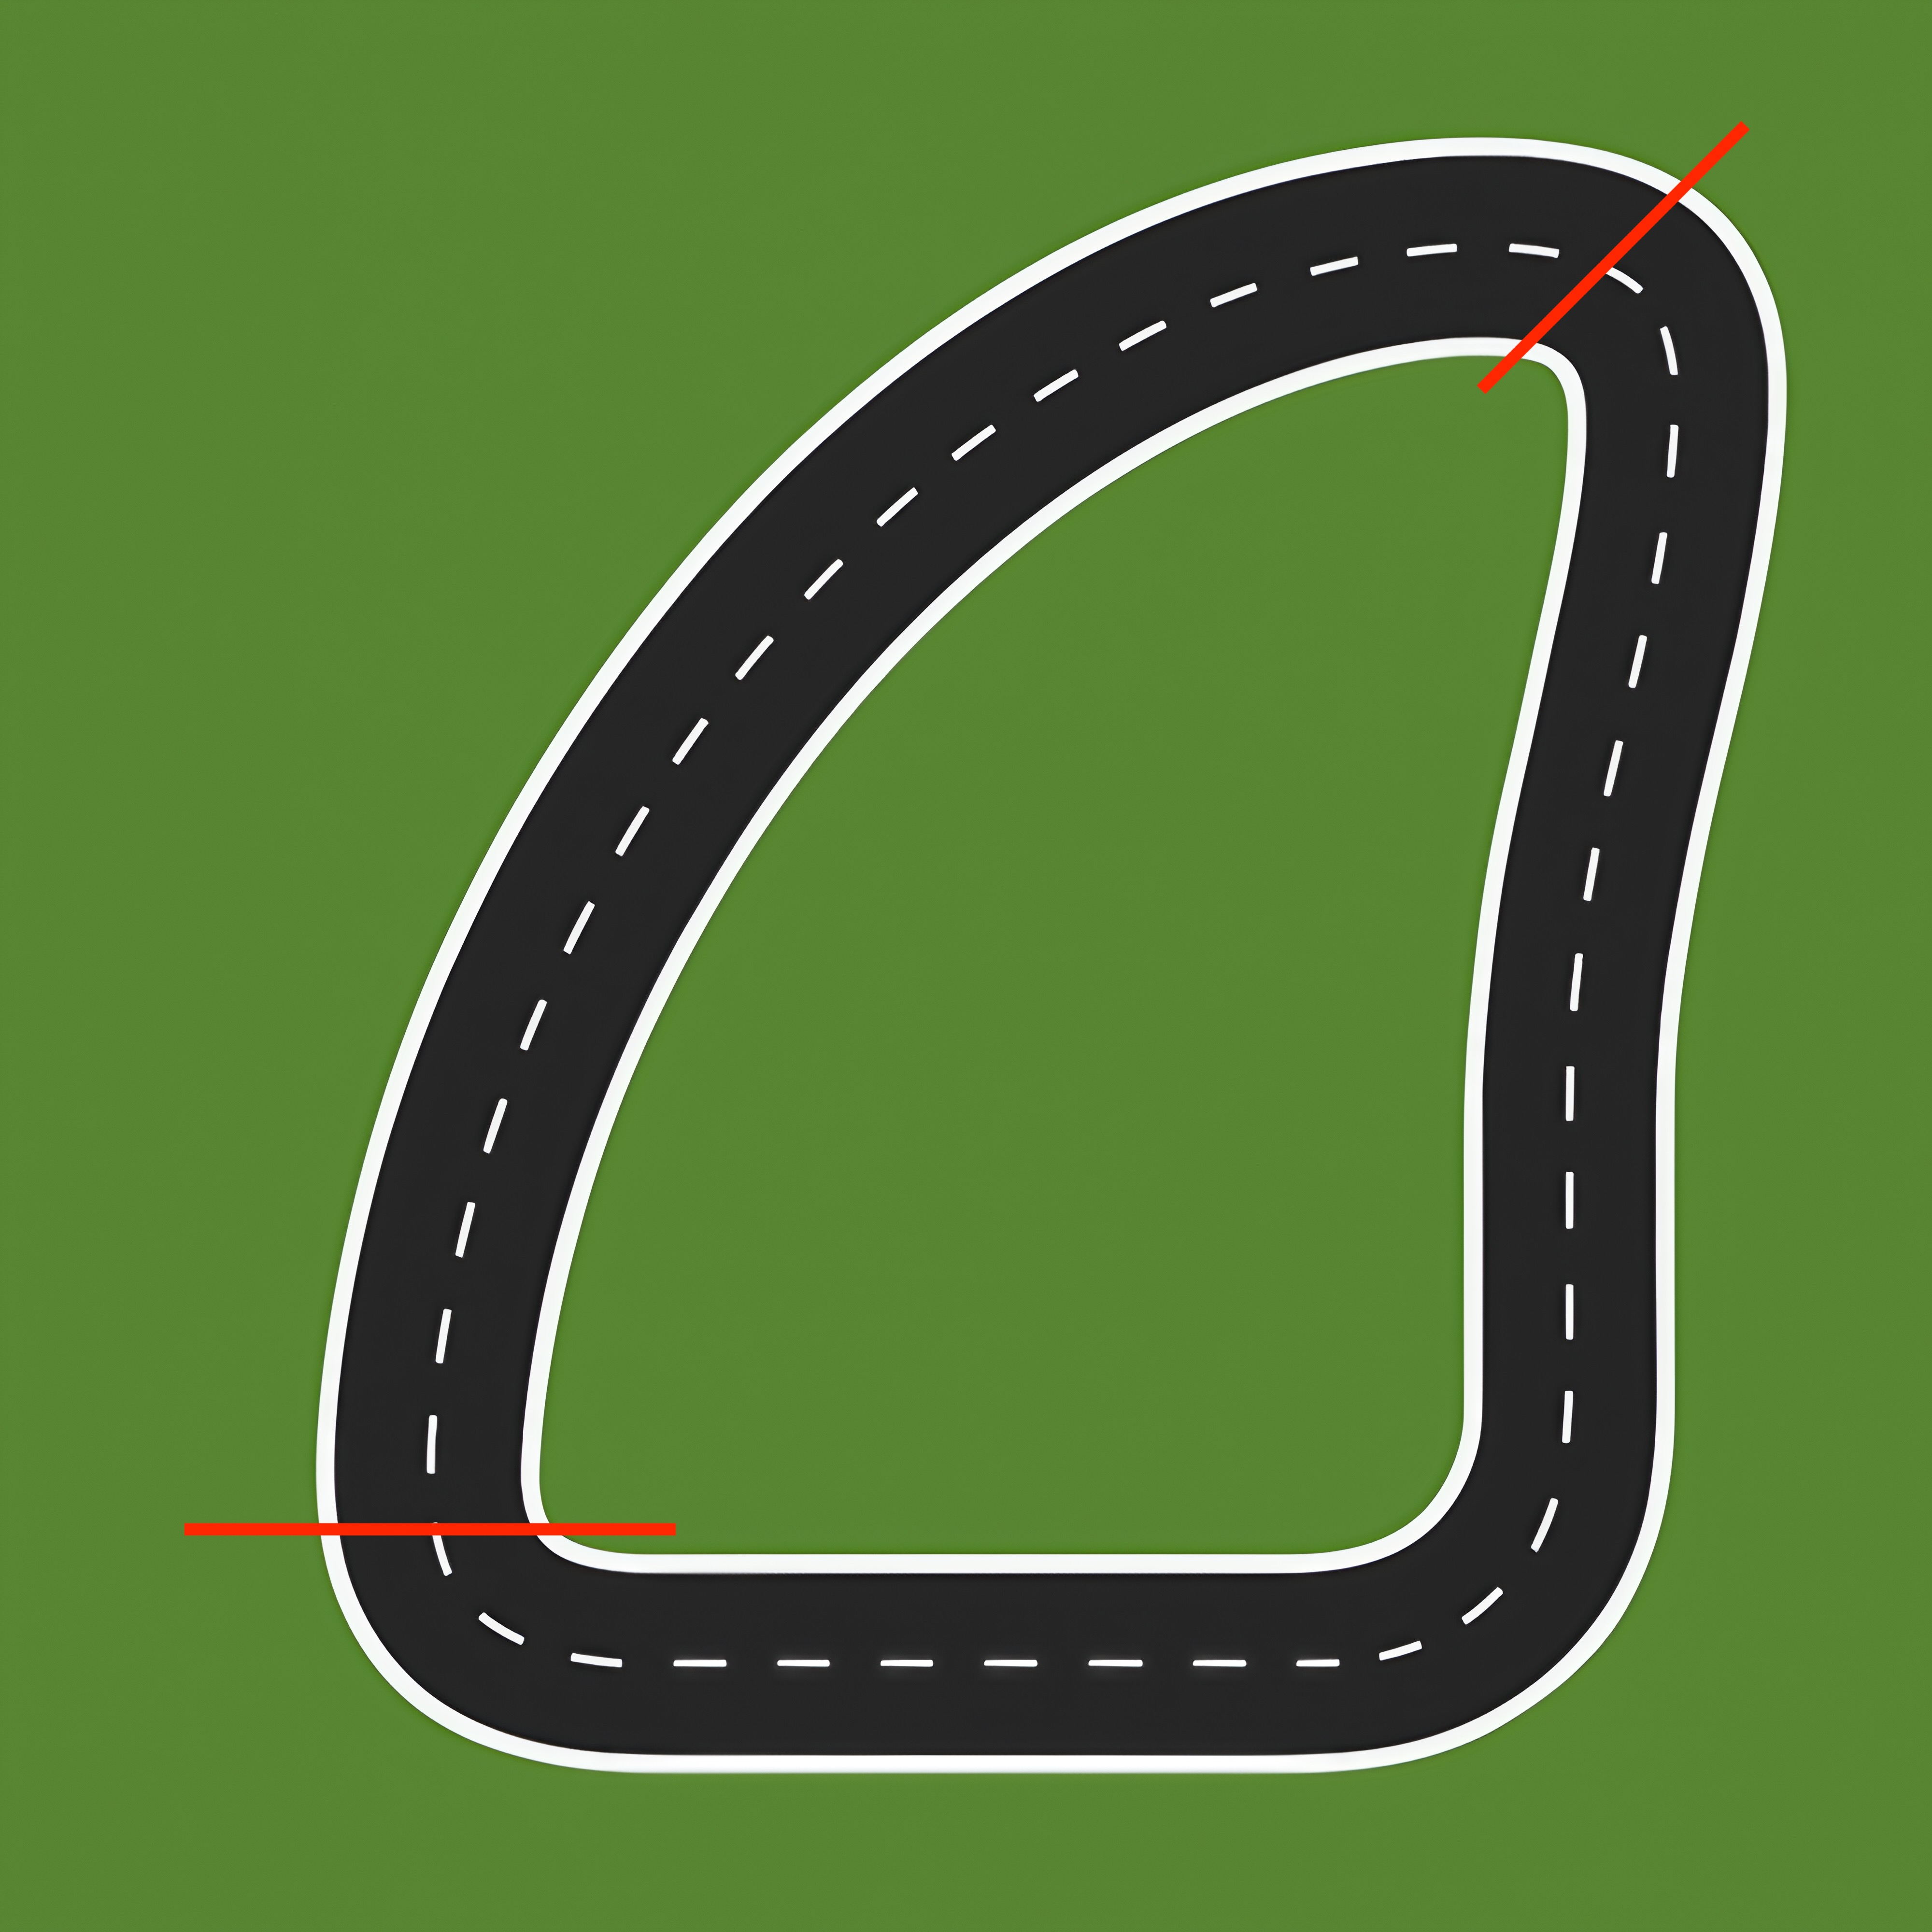
\includegraphics[width=\linewidth]{figures/Kurve.jpeg}
    \caption{Kurvenfahrt}
    \label{fig:kurvenfahrt}
  \end{wrapfigure}
  Die Fahrbahn ist als texturierte Ebene von 64m x 64m realisiert; die effektive Spurbreite beträgt an der 
  Referenzlinie etwa \SI{3.6}{\meter}. Die Strecke kombiniert eine lange Linkskurve (großer Radius) mit 
  einem engen Rechtsknick und eignet sich damit zur Bewertung von Spurtreue und Balance unter gekrümmter 
  Führung. Sofern nicht anders angegeben, sind für die Balance der \emph{PID}-Satz $K_p{=}2.0$, $K_i{=}0.2$, $K_d{=}0.5$, 
  der zulässige Lenkwinkelbereich $\delta\in[-0.3,\,0.3]\,\si{rad}$ 
  sowie $v_\text{base}{=}\SI{7}{km/h}$ (Grenzen \SI{5}{km/h} bis \SI{7}{km/h}) aktiv. 
  Mechanische Plausibilitätsgrenzen sind mit $\delta_\text{phys,max}{=}\SI{1.5}{rad}$ 
  und $\varphi_\text{roll,max}{=}45^\circ$ gesetzt. Für die visuelle Spurführung kann wahlweise 
  YOLO (Konfidenz 0{.}5) oder eine robuste ROI-Fallback-Erkennung verwendet werden (\texttt{roi\_top\_frac} = 0{.}5, 
  \texttt{roi\_height\_frac} = 0{.}06); Lenkbefehle werden durch \texttt{max\_delta} = 0{.}001 
  und \texttt{max\_steer\_cmd} = 0{.}06 geglättet und begrenzt. Ziel ist die Fahrt von der ersten 
  zur zweiten roten Markierung bei möglichst mittiger Spurhaltung und stabiler Balance.

  \paragraph{Einsatz eines vereinfachten Balance-P-Reglers}
  Für eine Baseline wurde der Balance-Regler auf einen reinen P-Anteil gesetzt ($K_p{=}2.0$, $K_i{=}0.0$, 
  $K_d{=}0.0$). \autoref{fig:kurvenfahrt-p} zeigt die gemessenen Größen der Fahrt, \autoref{fig:kurvenfahrt-p-error} 
  den zugehörigen ROI-Querfehler und \autoref{fig:kurvenfahrt-p-strecke} die Trajektorie auf der Strecke.
  \begin{figure}[H]
    \centering
    
\includegraphics[width=\textwidth]{figures/Kurve/Test P und PID/P/Daten.png}
    \caption{Kurvenfahrt mit reinem P-Regler (Zeitreihen)}
    \label{fig:kurvenfahrt-p}
  \end{figure}
  Bereits nach wenigen Sekunden setzt ein wachsendes Aufschaukeln ein: Der durch den Rollwinkel 
  induzierte Stellbefehl (\texttt{final\_steer}) treibt den Lenkeinschlag alternierend nach links/rechts, 
  bis die Phasenreserve erschöpft ist. Infolge der reinen Proportionalrückführung, der Aktuatorbegrenzungen 
  und der unvermeidlichen Latenzen entsteht ein unterdämpftes Verhalten; das Fahrrad kippt nach rund \SI{15}{\second} nach rechts.
  \begin{figure}[H]
    \centering
    
\includegraphics[width=\textwidth]{figures/Kurve/Test P und PID/P/Error.png}
    \caption{ROI-Querfehler während der P-Regler-Fahrt}
    \label{fig:kurvenfahrt-p-error}
  \end{figure}


  \begin{wrapfigure}{r}{0.40\textwidth}
    \vspace{-0.8\baselineskip}
    \centering
    
\includegraphics[width=\linewidth]{figures/Kurve/Test P und PID/P/Strecke.png}
    \caption{Gefahrene Trajektorie (P-Regler)}
    \label{fig:kurvenfahrt-p-strecke}
  \end{wrapfigure}


  Der ROI-Querfehler zeigt eine ausgeprägte Kopplung zum Rollwinkel: Das Pendeln der Balance überträgt sich 
  phasenverschoben auf die seitliche Abweichung. Zur Stabilisierung ist daher ein kleiner Integralanteil 
  (Elimination stationärer Abweichung mit Anti-Windup) und insbesondere ein Derivativanteil (Phasenführung/Dämpfung) 
  erforderlich; in Kombination mit Rate(\texttt{max\_delta}) und Amplitudenbegrenzung (\texttt{max\_steer\_cmd}) 
  wird das Überschwingen reduziert und ein Kippen verhindert.

  \clearpage
  \paragraph{Einsatz des erweiterten Balance-PID-Reglers}
  Für diese Versuchsfahrt wurden die erweiterten PID-Parameter $K_p = 2.0$, $K_i = 0.2$ und $K_d = 0.5$ eingesetzt. 
  Die Spurführung erfolgte mittels YOLO-basierter Bildverarbeitung. Während die Parameterwahl eine Verbesserung der 
  Stabilität gegenüber reinen P-Reglern bewirkte, zeigte sich nach etwa 35 s dennoch ein Kippen des Fahrrads, 
  ausgelöst durch abrupte Richtungsänderungen in der vom Vision-Modell vorgegebenen Trajektorie.
  \begin{figure}[H]
    \centering
    
\includegraphics[width=\textwidth]{figures/Kurve/Test P und PID/YOLO PID/Daten.png}
    \caption{Kurvenfahrt mit PID-Regler und YOLO-Spurführung}
    \label{fig:kurvenfahrt-pid-yolo}
  \end{figure}
  
  Die Fehleranalyse bestätigt, dass die Fahrbahnerkennung zum Zeitpunkt der Versuche noch unzureichend trainiert war. 
  Ab Sekunde 31 steigt der Querfehler abrupt an und fällt kurz darauf wieder ab (Sekunde 34). Dieses unstete Verhalten 
  überträgt sich auf den Rollwinkel, dessen zunehmendes Pendeln schließlich eskaliert und zum Umkippen des Fahrrads nach rechts führt.
  
  \begin{figure}[H]
    \centering
    
\includegraphics[width=\textwidth]{figures/Kurve/Test P und PID/YOLO PID/Error.png}
    \caption{ROI-Querfehler während der PID-Regler-Fahrt (YOLO)}
    \label{fig:kurvenfahrt-pid-error-yolo}
  \end{figure}

  \begin{wrapfigure}{r}{0.40\textwidth}
    \vspace{-0.8\baselineskip}
    \centering
    
\includegraphics[width=\linewidth]{figures/Kurve/Test P und PID/YOLO PID/Strecke.png}
    \caption{Gefahrene Trajektorie (PID-Regler mit YOLO)}
    \label{fig:kurvenfahrt-pid-strecke-yolo}
  \end{wrapfigure}

  Trotz dieser Limitierungen lässt sich durch die Kombination von Integral- und Differentialanteil eine verbesserte Spurhaltung 
  mit reduzierten Querabweichungen beobachten. Insbesondere werden stationäre Fehler kompensiert und Überschwinger wirksam gedämpft, 
  sodass das Fahrrad über weite Teile der Strecke stabil bleibt – auch bei eingeschränkter Fahrbahnerkennung. Kurz vor dem Ziel 
  versagt die Kompensation jedoch, und das System verliert seine Stabilität. Dies verdeutlicht, dass die Reglererweiterung eine 
  deutliche Verbesserung bewirkt, die Robustheit aber maßgeblich von der Qualität der visuellen Erkennung abhängt.

  \clearpage

  Die Abbildungen 24a und 24b verdeutlichen Limitierungen der \emph{YOLO}-Segmentierung: Abschnitte der Fahrbahn werden 
  nur teilweise bzw.\ falsch klassifiziert; insbesondere die Trennung zwischen Fahrbahn und Nebenflächen (z.\,B.\ Rand-/Grünstreifen) 
  ist inkonsistent. Links (a) ist die Spur weitgehend korrekt maskiert, rechts (b) werden Randbereiche fälschlich als Straße erkannt. 
  Diese Fehlklassifikationen verschieben die geschätzte Spurmitte, erzeugen sprunghafte Querfehler und können instabile Lenkbefehle auslösen.


  \begin{figure}[H]
    \centering
    \begin{subfigure}[t]{0.48\textwidth}
      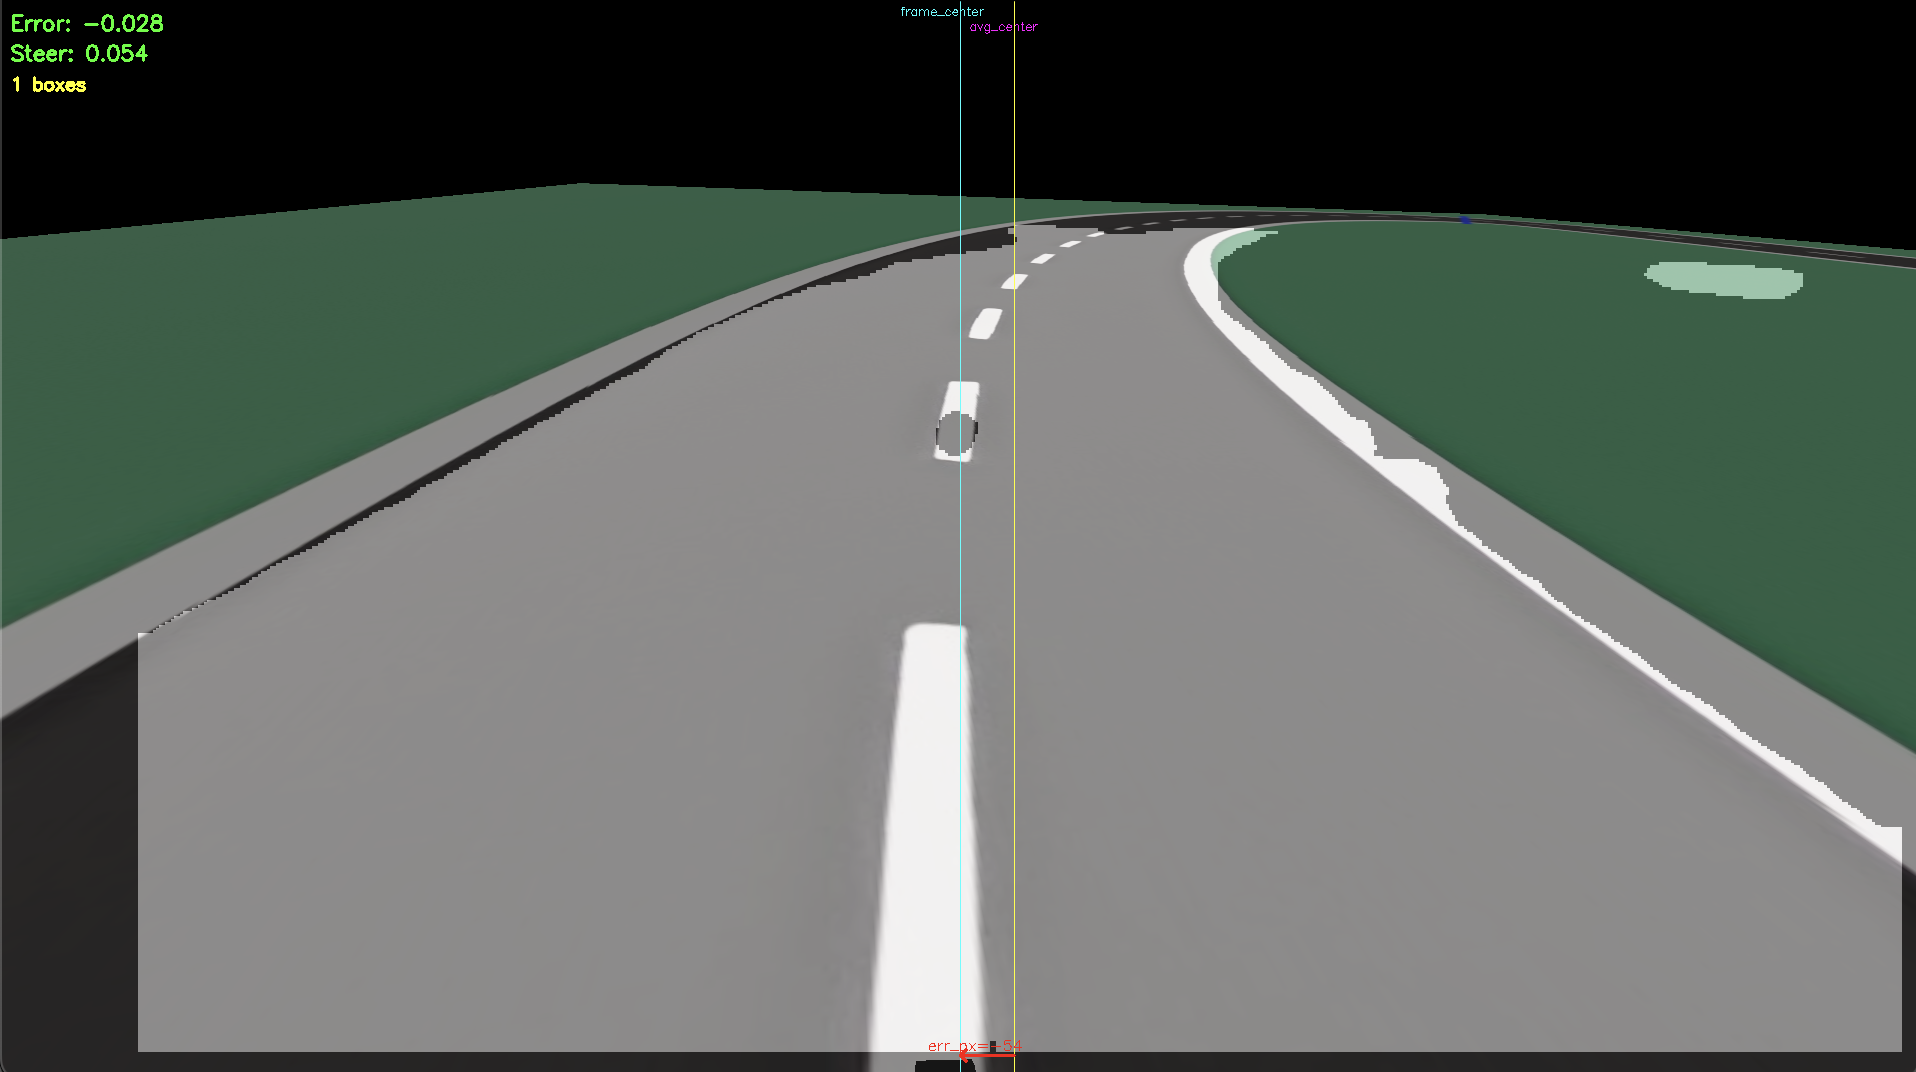
\includegraphics[width=\linewidth]{figures/Kurve/Test P und PID/YOLO PID/Strecke gut.png}
      \caption{Strecke gut}\label{fig:strecke-gut}
    \end{subfigure}\hfill
    \begin{subfigure}[t]{0.48\textwidth}
      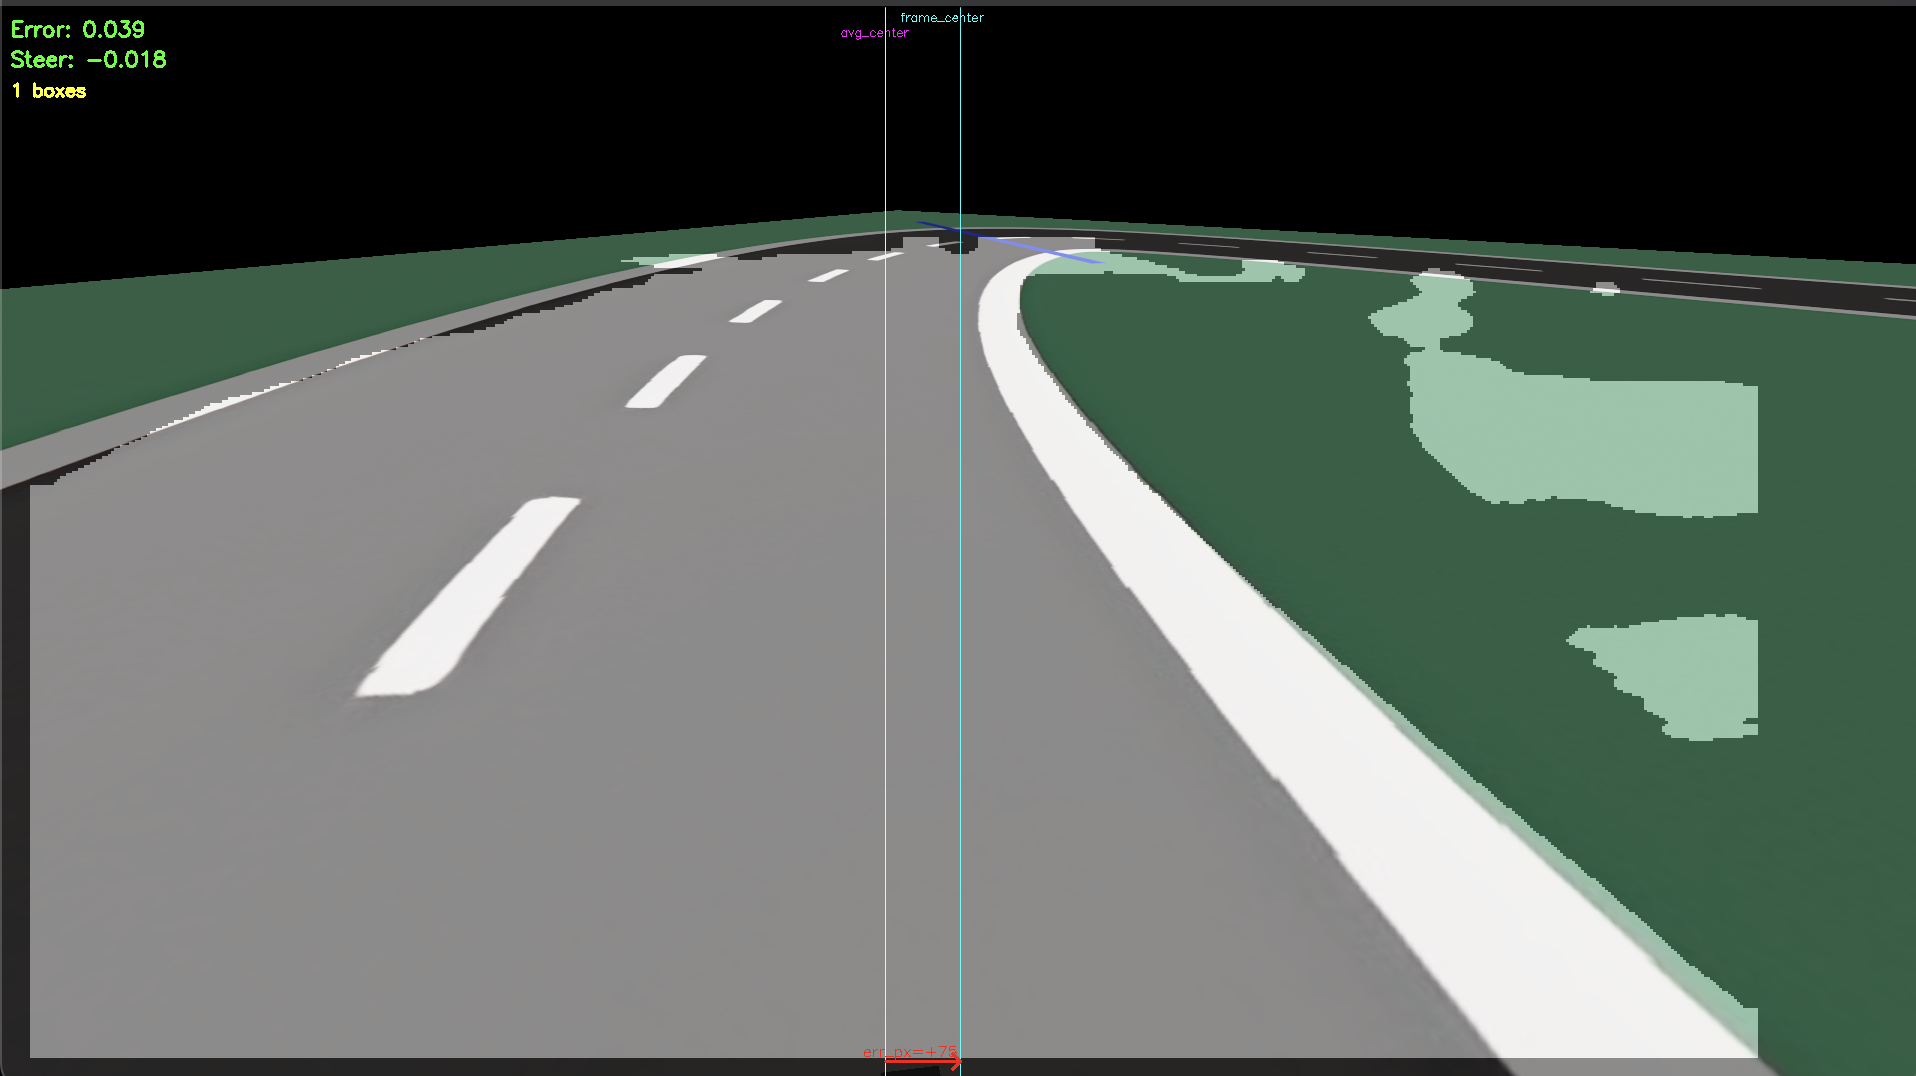
\includegraphics[width=\linewidth]{figures/Kurve/Test P und PID/YOLO PID/Stecke schlecht.png}
      \caption{Strecke schlecht}\label{fig:strecke-schlecht}
    \end{subfigure}
    \caption{Strecke gut und schlecht nebeneinander.}\label{fig:strecke-gut-schlecht}
  \end{figure}


  \paragraph{Einsatz der ROI\mbox{-}Fallback\mbox{-}Erkennung}
  In dieser Versuchsfahrt wurde die ROI\mbox{-}Fallback\mbox{-}Erkennung eingesetzt, um die in Abschnitt~4.3.1 beschriebenen Schwächen der \emph{YOLO}-Segmentierung zu umgehen. Die Pipeline nutzt klassische Bildverarbeitung innerhalb eines definierten Bildausschnitts (ROI): farbbasierte Segmentierung der Fahrbahn und Kantenfilter werden kombiniert, die Spurmittellinie wird aus der ROI-Maske abgeleitet und zeitlich geglättet. Sämtliche Reglerparameter (\emph{PID}) sowie die übrigen Versuchsbedingungen entsprechen exakt denen der YOLO-Konfiguration; die beobachteten Unterschiede sind daher allein auf die Wahrnehmung (Erkennung) zurückzuführen.
  
  \begin{figure}[H]
    \centering
    
\includegraphics[width=\textwidth]{figures/Kurve/Test P und PID/PID/Daten.png}
    \caption{Kurvenfahrt mit PID\mbox{-}Regler und ROI\mbox{-}Fallback\mbox{-}Erkennung}
    \label{fig:kurvenfahrt-pid-strecke-roi}
  \end{figure}
  
  Die Ergebnisse in \autoref{fig:kurvenfahrt-pid-strecke-roi} zeigen einen deutlichen Qualitätsgewinn gegenüber der YOLO\mbox{-}Erkennung: sprunghafte Querfehler treten praktisch nicht mehr auf, und das Fahrrad fährt über weite Strecken stabil. Kurzzeitige Anregungen (z.\,B.\ zwischen Sekunde~20 und~25) führen zwar zu einer temporären Erhöhung der Stellgrößen, werden jedoch vom PID\mbox{-}Regler sauber kompensiert. Der anfängliche Anstieg des \emph{Final\mbox{-}Steer} ist auf das Einfädeln in die Spur zurückzuführen; nach kurzer Transiente regelt sich das System auf einen kleinen stationären Fehler ein.
  
  \begin{figure}[H]
    \centering
    
\includegraphics[width=\textwidth]{figures/Kurve/Test P und PID/PID/Error.png}
    \caption{ROI\mbox{-}Querfehler während der PID\mbox{-}Regler\mbox{-}Fahrt (ROI)}
    \label{fig:kurvenfahrt-pid-error-roi}
  \end{figure}
  
  \begin{wrapfigure}{r}{0.40\textwidth}
    \vspace{-0.8\baselineskip}
    \centering
    
\includegraphics[width=\linewidth]{figures/Kurve/Test P und PID/PID/Strecke.png}
    \caption{Gefahrene Trajektorie (PID\mbox{-}Regler, ROI)}
    \label{fig:kurvenfahrt-pid-strecke}
  \end{wrapfigure}
  
  Im Fehlerverlauf (\autoref{fig:kurvenfahrt-pid-error-roi}) ist außerdem ersichtlich, dass ab etwa Sekunde~35 die (rote) Schwelle zur scharfen Kurve überschritten wird und der Querfehler ansteigt. Dieses Verhalten ist konsistent mit den in der Regelkette gesetzten Lenkwinkel- und Ratenbegrenzungen (\texttt{max\_steer\_cmd}, \texttt{max\_delta}): Bei hoher Streckenkrümmung gerät der Regler kurzzeitig in Sättigung, bevor der Fehler wieder abgebaut wird. Die zugehörige Trajektorie (\autoref{fig:kurvenfahrt-pid-strecke}) belegt dennoch eine insgesamt mittige und ruhige Spurhaltung; Abweichungen konzentrieren sich auf den Scheitel der Kurve und bleiben begrenzt.
  
  \smallskip
  \noindent\textit{Fazit.} Die ROI\mbox{-}Fallback\mbox{-}Erkennung erhöht die Robustheit der Spurführung, indem sie Ausreißer in der visuellen Messung reduziert und so die Kopplung zum Balance\mbox{-}Regelkreis entlastet. Ihre Wirksamkeit ist allerdings an Szenen mit gut trennbaren Fahrbahn-/Nebenflächen gebunden; für variable Beleuchtung, Texturen oder komplexe Hintergründe ist eine verbesserte (oder zusätzlich trainierte) lernbasierte Segmentierung weiterhin wünschenswert.
  

  \newpage

  






  %------------------------------------------------------------------------------------------------
  %------------------------------------------------------------------------------------------------

  \subsubsection{S-Kurve}


    \begin{figure}[H]
      \centering
      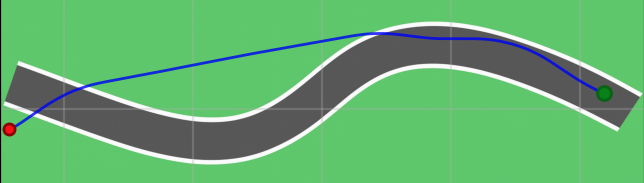
\includegraphics[width=1.0\textwidth]{figures/S-Kurve/Yolo_Strecke.png}  
      \caption{Fallback Strecke S-Kurve}
      \label{fig:fallback-strecke-s-kurve}
    \end{figure}

    \begin{figure}[H]
      \centering
      
\includegraphics[width=1.0\textwidth]{figures/S-Kurve/Fallback_Strecke.png}  
      \caption{Fallback Strecke S-Kurve}
      \label{fig:fallback-strecke-s-kurve}
    \end{figure}

   
    \begin{figure}[H]
      \centering
      
\includegraphics[width=1.0\textwidth]{figures/S-Kurve/Yolo_Daten.png}  
      \caption{YOLO Daten S-Kurve}
      \label{fig:yolo-daten-s-kurve}
    \end{figure}
  
    \begin{figure}[H]
      \centering
      
\includegraphics[width=1.0\textwidth]{figures/S-Kurve/Yolo_Error.png}  
      \caption{Error YOLO S-Kurve}
      \label{fig:yolo-error-s-kurve}
    \end{figure}

    

    \begin{figure}[H]
      \centering
      
\includegraphics[width=1.0\textwidth]{figures/S-Kurve/Fallback_Daten.png}  
      \caption{Fallback Strecke S-Kurve}
      \label{fig:fallback-strecke-s-kurve}
    \end{figure}

    \begin{figure}[H]
      \centering
      
\includegraphics[width=1.0\textwidth]{figures/S-Kurve/Fallback_Error.png}  
      \caption{Fallback Strecke S-Kurve}
      \label{fig:fallback-strecke-s-kurve}
    \end{figure}

    

   

   



    %------------------------------------------------------------------------------------------------
    %------------------------------------------------------------------------------------------------






  \subsubsection{Gerade Strecke mit Seitenwind}




  %------------------------------------------------------------------------------------------------
  %------------------------------------------------------------------------------------------------
  \subsubsection{Gerande Stecke mit Höhenunterschied}

  \begin{figure}[H]
    \centering
    \begin{subfigure}[t]{0.48\textwidth}
      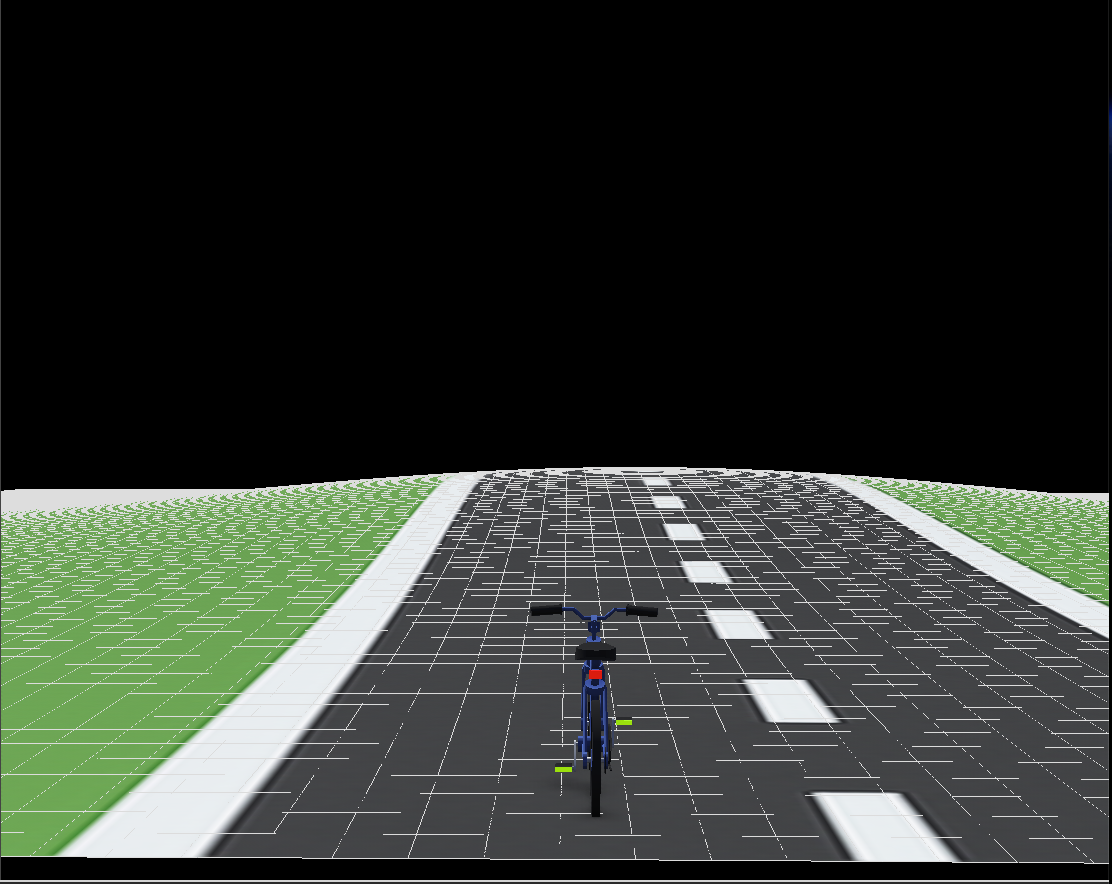
\includegraphics[width=\linewidth]{figures/Huegel.png}
      \caption{Hügel}\label{fig:huegel}
    \end{subfigure}\hfill
    \begin{subfigure}[t]{0.48\textwidth}
      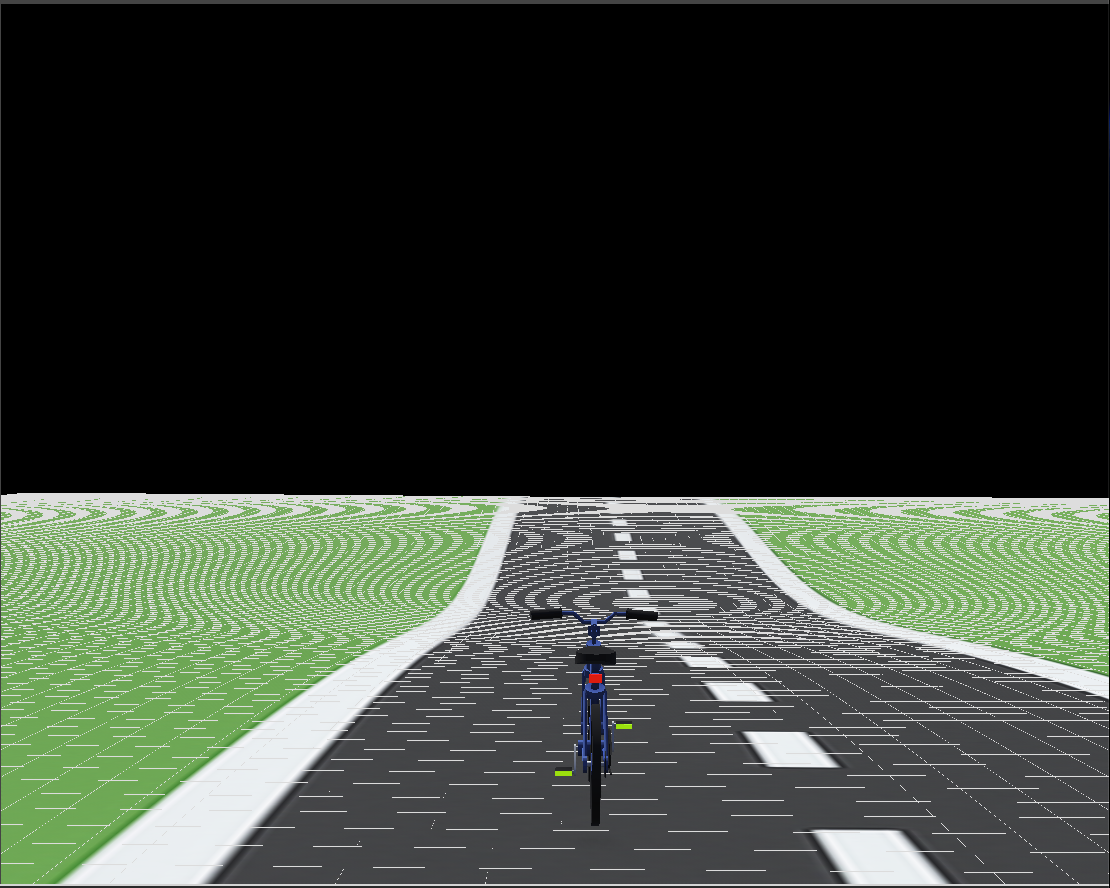
\includegraphics[width=\linewidth]{figures/Tunnel.png}
      \caption{Tunnel}\label{fig:tunnel}
    \end{subfigure}
    \caption{Hügel und Tunnel nebeneinander.}\label{fig:huegel-tunnel}
  \end{figure}
  

  %------------------------------------------------------------------------------------------------
  %------------------------------------------------------------------------------------------------

\subsection{Balance-Stabilität}
\subsection{Spurtreue \& Querabweichung}
\subsection{Rechenzeit \& Echtzeitfähigkeit}
\newpage
